%---------------------导言区---------------------------%
\documentclass[12pt,a4paper,UTF8]{ctexart}
\usepackage{geometry}
	\geometry{left=2.5cm,right=2.5cm,top=3.2cm,bottom=2.8cm}
\usepackage{xeCJK,amsmath,paralist,enumitem,booktabs,multirow,graphicx,subfig,setspace,listings,lastpage}
	\setlength{\parindent}{2em}
	\lstset{language=Python}
\usepackage{fancyhdr}
	\pagestyle{fancy}
	\rhead{C1 密里根油滴实验测量元电荷}
	\lhead{基础物理实验\uppercase\expandafter{\romannumeral2}简要实验报告}
	\cfoot{Page \thepage/\pageref{LastPage}}  %当前页\总页数
	\rfoot{\today}
	\renewcommand{\headrulewidth}{0.4pt}
	\renewcommand{\theenumi}{(\arabic{enumi})}
\usepackage[colorlinks,linkcolor=blue,urlcolor=blue,citecolor=blue]{hyperref}
%%%%%%%%%%%%%%%%%%%%%%%%%%%%%%%%%%%%%%%%%%%%%%%%%%%%%%%%%%
%%%%%%%%%%%%%%%%%%%%%%%%%正文开始%%%%%%%%%%%%%%%%%%%%%%%%%%
%%%%%%%%%%%%%%%%%%%%%%%%%%%%%%%%%%%%%%%%%%%%%%%%%%%%%%%%%%

\begin{document}

%%begin-------------------标题与信息-----------------------%%
%%标题
\begin{center}
\LARGE\textbf{C1 密里根油滴实验测量元电荷}
\end{center}

%%信息
\begin{doublespacing}
	\centering
	\begin{tabular}{ll}
	 & \\
	{\CJKfontspec{Droid Sans Fallback} 实验人:黄子维 20980066} & {\CJKfontspec{Droid Sans Fallback}合作者:黄睿杰 20980062}\\
	{\CJKfontspec{Droid Sans Fallback} 实验时间:2021.12.16~星期四~上午} & {\CJKfontspec{Droid Sans Fallback} 室温:22$^{\circ}$C~相对湿度:77\%}
	\end{tabular}
\end{doublespacing}
%%end-------------------标题与信息-----------------------%%

\subsection*{【数据处理及分析】}
    实验参数如表\ref{tab:0}
    \begin{table}[htbp]
        \centering
            \begin{tabular}{cc}
                \toprule
                参数	&值    \\
                \midrule
                $d$    &$5 \times 10^{-3} m$    \\
                $\eta$    &$1.83 \times 10^{-5} kg/(m \cdot s)$    \\
                $b$    &$6.17 \times 10^{-6} m/cmHg$   \\
                $l$    &$1.6 mm$   \\
                $g$    &$9.78858 m/s^2$    \\
                $\rho$    &$981 kg/m^3$    \\
                $p$    &$76.0 cmHg$    \\
                \bottomrule
            \end{tabular}
            \caption{\textbf{实验参数}}
            \label{tab:0}
    \end{table}

    \subsubsection*{1. 静态法}
    \paragraph{静态法测量元电荷原理}
    \newline
	\indent
    选取合适油滴,测量油滴平衡电压$U$和油滴在重力和空气阻力作用下匀速下落时间$t_g$。
    代入公式\ref{eq:1},可以计算油滴电荷量$q$。
    将油滴电荷量$q$除以元电荷公认值$e = 1.60217733 \times 10^{-19} C$,并取最邻近整数,可以计算油滴带电子数$n$。
    线性拟合$q(n)$,直线斜率即为实验测量元电荷值$e_{exp} = k$。
    相对误差为$\frac{e-e_{exp}}{e} \times 100\%$。
    \begin{align}
        q &= \frac{18\pi}{\sqrt{2\rho g}}\left[\frac{\eta l}{t_g \left(1+\frac{b}{pa}\right) }\right]^{3/2} \frac{d}{V} \\
        a &= \sqrt{\frac{9\eta l}{2t_g\rho g}}
        \label{eq:1}
    \end{align}

    \paragraph{实验结果}
    \newline
	\indent
    实验共选取五个油滴,每个油滴重复测量五次。
    $U$和$t_g$取为每个油滴重复测量数据平均值,
    并计算A类不确定度$S_A$、B类不确定度$S_B$以及合成不确定度$S$。
    其余参量见表\ref{tab:0}。
    
    油滴电荷量和带电子数如表\ref{tab:1.1},电荷量不确定度见计算代码文件。
    拟合计算元电荷结果如\ref{fig:1}
    \begin{table}[htbp]
        \centering
            \begin{tabular}{cccccc}
                \toprule
                油滴    &下落时间$t_g /s$	&平衡电压$U/V$    &带电量$q/10^{-19}C$ &$q/e$  &电子数$n$  \\
                \midrule
                A   &17.24  &270.6	&$4.6 \pm 0.1$   &2.9   &3.0   \\
                B   &17.32	&262.6	&$4.7 \pm 0.1$   &3.0   &3.0   \\
                C   &30.55	&334.2	&$1.5 \pm 0.02$  &1.0   &1.0   \\
                D   &22.49	&129.2	&$6.4 \pm 0.05$  &4.0   &4.0   \\
                E   &31.51	&156.0	&$3.1 \pm 0.05$  &2.0   &2.0   \\
                \bottomrule
            \end{tabular}
            \caption{\textbf{静态法油滴电荷量和带电子数}}
            \label{tab:1.1}
    \end{table}

    \begin{figure}[htbp]
        \centering
        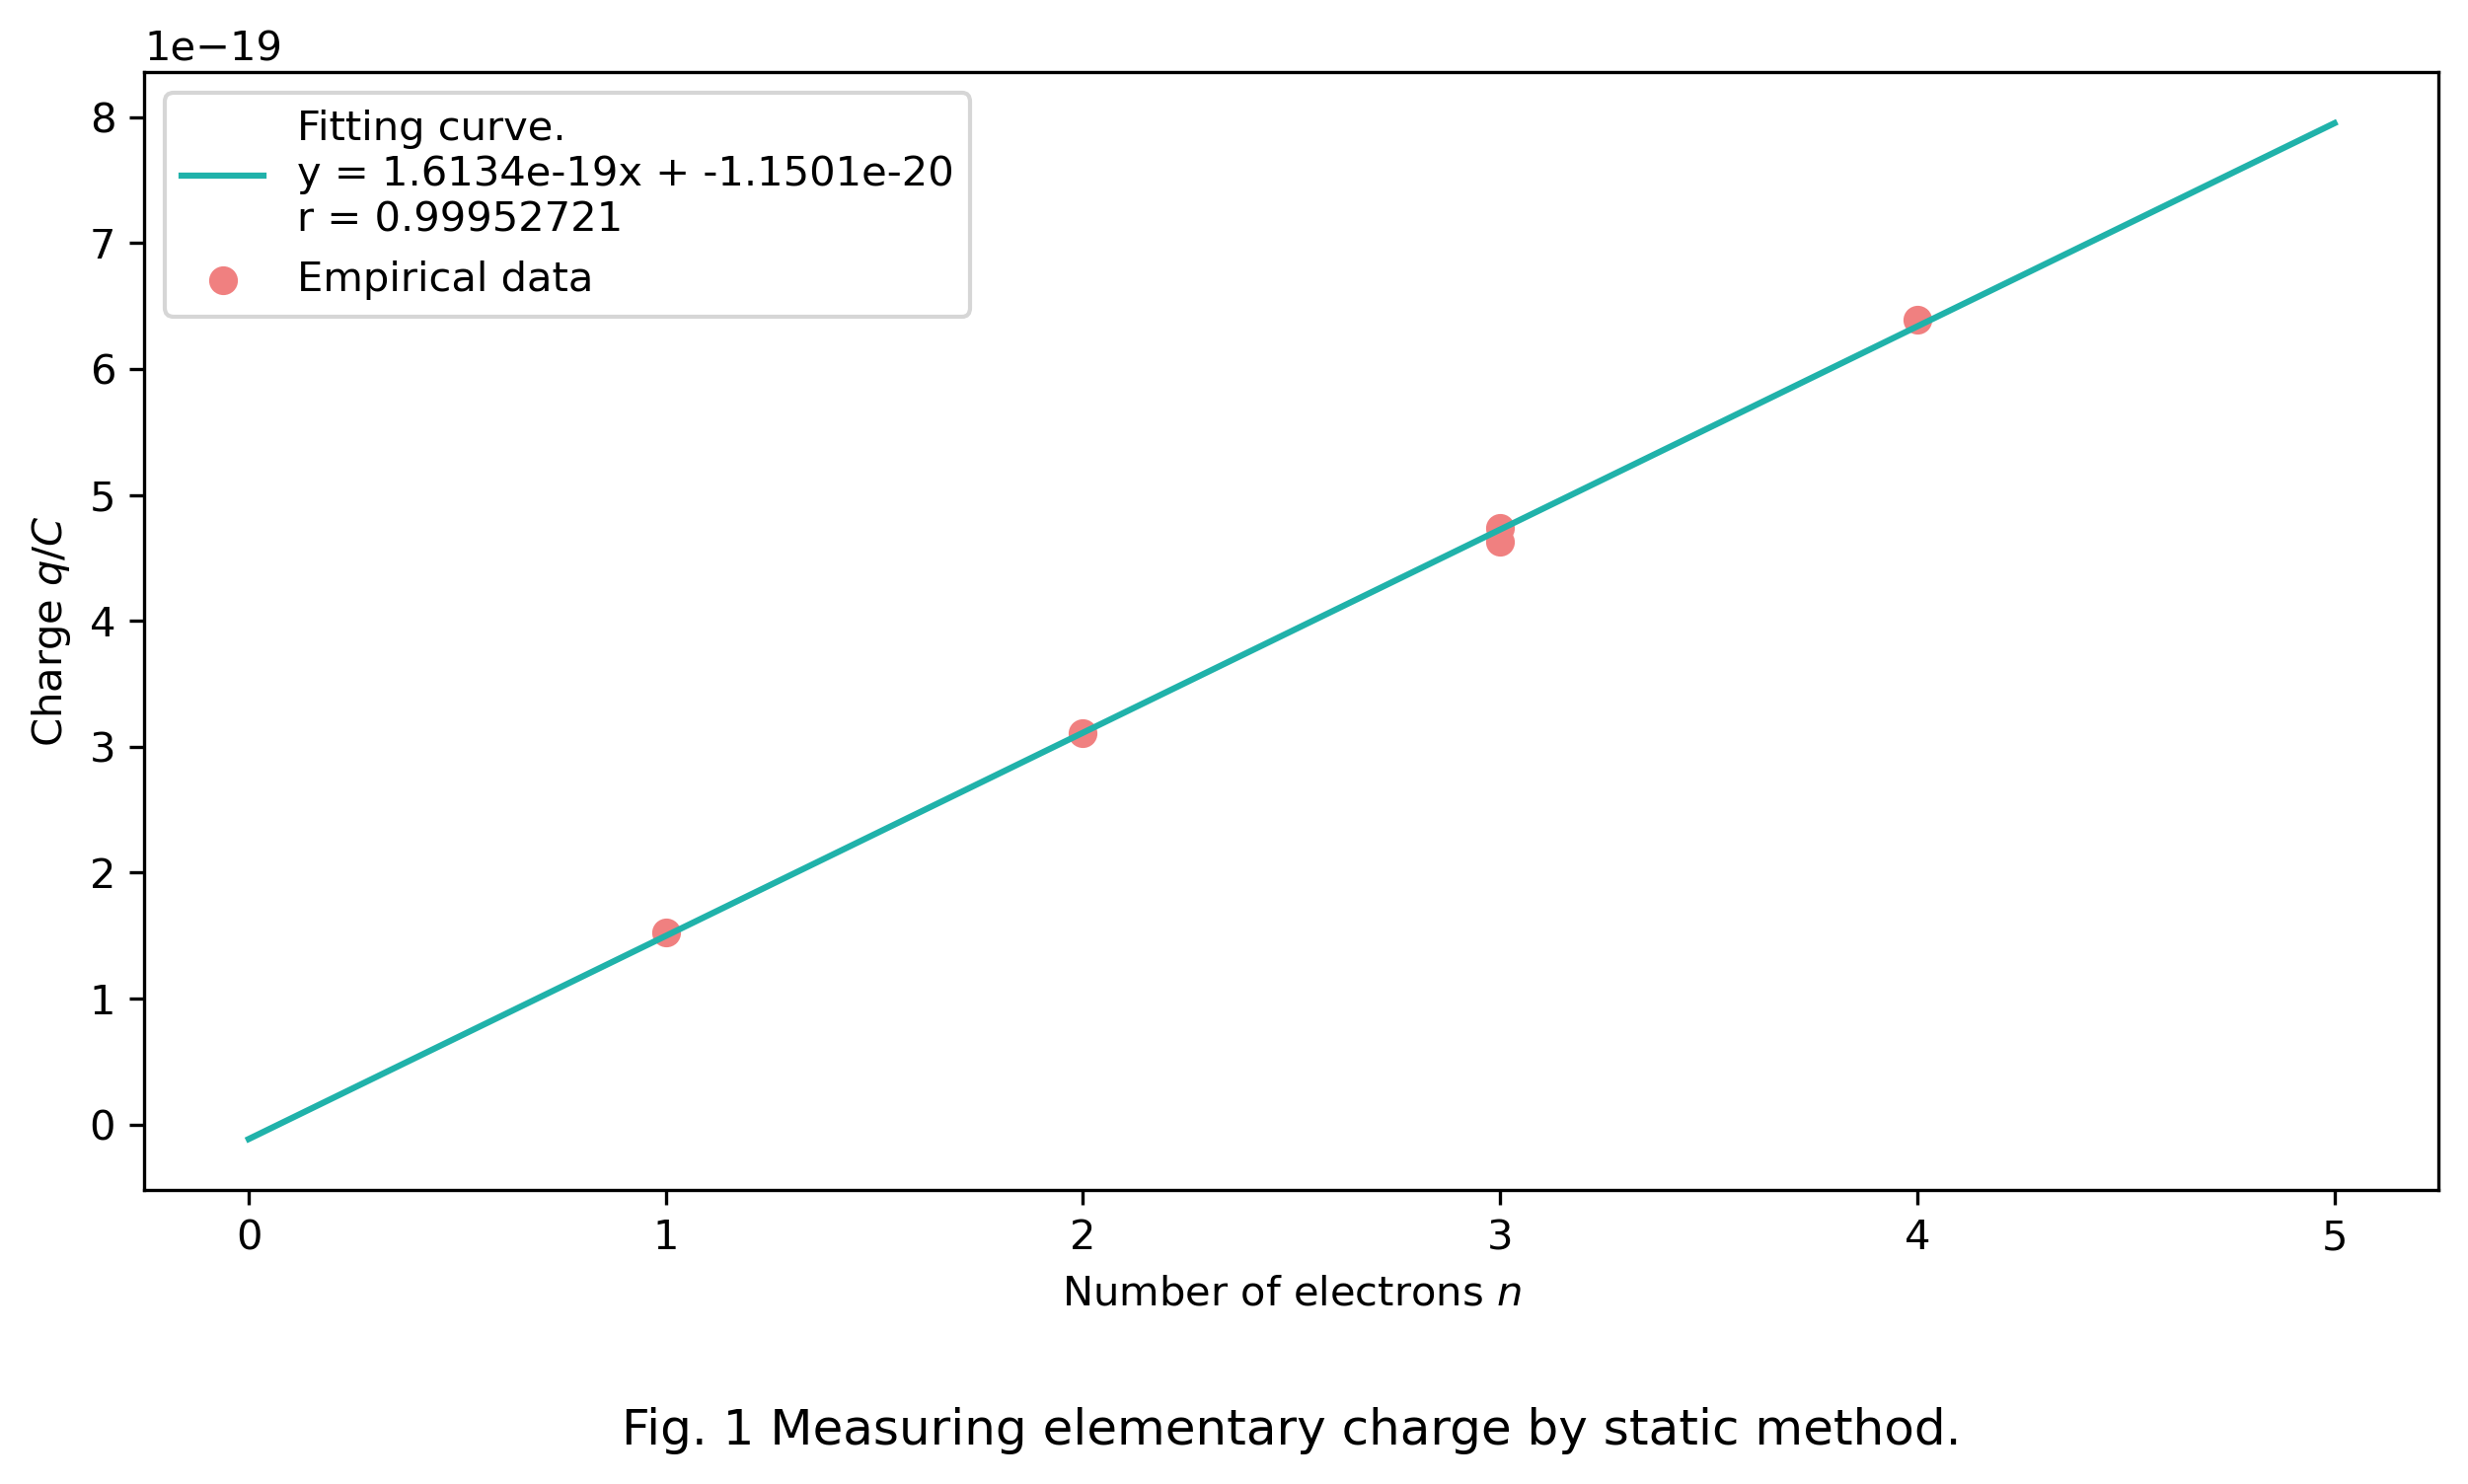
\includegraphics[width=0.7\textwidth]{attachments/fig.1.png}
        \caption{静态法拟合计算元电荷}
        \label{fig:1}
    \end{figure}

    拟合相关系数$r>0.99$,拟合效果好。
    元电荷测量值等于直线斜率$e = 1.61 \times 10^{-19} C$,相对误差为$0.7\%$。

    \subsubsection*{2. 动态法}
    \paragraph{动态法测量元电荷原理}
    \newline
	\indent
    给定合适电压,选取合适油滴,测量油滴在工作电压作用下上升时间$t_e$和油滴在重力和空气阻力作用下匀速下落时间$t_g$。
    代入公式\ref{eq:2},可以计算油滴电荷量$q$。
    将油滴电荷量$q$除以元电荷公认值$e = 1.60217733 \times 10^{-19} C$,并取最邻近整数,可以计算油滴带电子数$n$。
    线性拟合$q(n)$,直线斜率即为实验测量元电荷值$e_{exp} = k$。
    相对误差为$\frac{e-e_{exp}}{e} \times 100\%$。
    \begin{align}
        q &= \frac{18\pi}{\sqrt{2\rho g}}\left[\frac{\eta l}{\left(1+\frac{b}{pa}\right) }\right]^{3/2} \frac{d}{V} \left(\frac{1}{t_e}+\frac{1}{t_g}\right) \left(\frac{1}{t_g}\right)^{1/2} \\
        a &= \sqrt{\frac{9\eta l}{2t_g\rho g}}
        \label{eq:2}
    \end{align}

    \paragraph{实验结果}
    \newline
	\indent
    实验共选取五个油滴,每个油滴重复测量五次。
    $t_e$和$t_g$取为每个油滴重复测量数据平均值,
    并计算A类不确定度$S_A$、B类不确定度$S_B$以及合成不确定度$S$。
    其余参量见表\ref{tab:0}。
    
    油滴电荷量和带电子数如表\ref{tab:2.1},电荷量不确定度见计算代码文件。
    拟合计算元电荷结果如\ref{fig:2}
    \begin{table}[htbp]
        \centering
            \begin{tabular}{ccccccc}
                \toprule
                油滴    &上升时间$t_e /s$   &下落时间$t_g /s$	&工作电压$U/V$    &带电量$q/10^{-19}C$ &$q/e$  &电子数$n$  \\
                \midrule
                A   &12.40   &30.61 &196.0	&$9.0 \pm 0.2$  &5.6   &6.0   \\
                B   &11.24   &30.29	&250.0	&$7.6 \pm 0.2$  &4.8   &5.0   \\
                C   &28.53   &23.66	&300.0	&$4.6 \pm 0.2$  &2.9   &3.0   \\
                D   &10.59   &21.52	&356.0	&$7.5 \pm 0.1$  &4.7   &5.0   \\
                E   &12.65   &21.24	&150.0	&$1.6 \pm 0.2$  &10.0   &10.0   \\
                \bottomrule
            \end{tabular}
            \caption{\textbf{动态法油滴电荷量和带电子数}}
            \label{tab:2.1}
    \end{table}

    \begin{figure}[htbp]
        \centering
        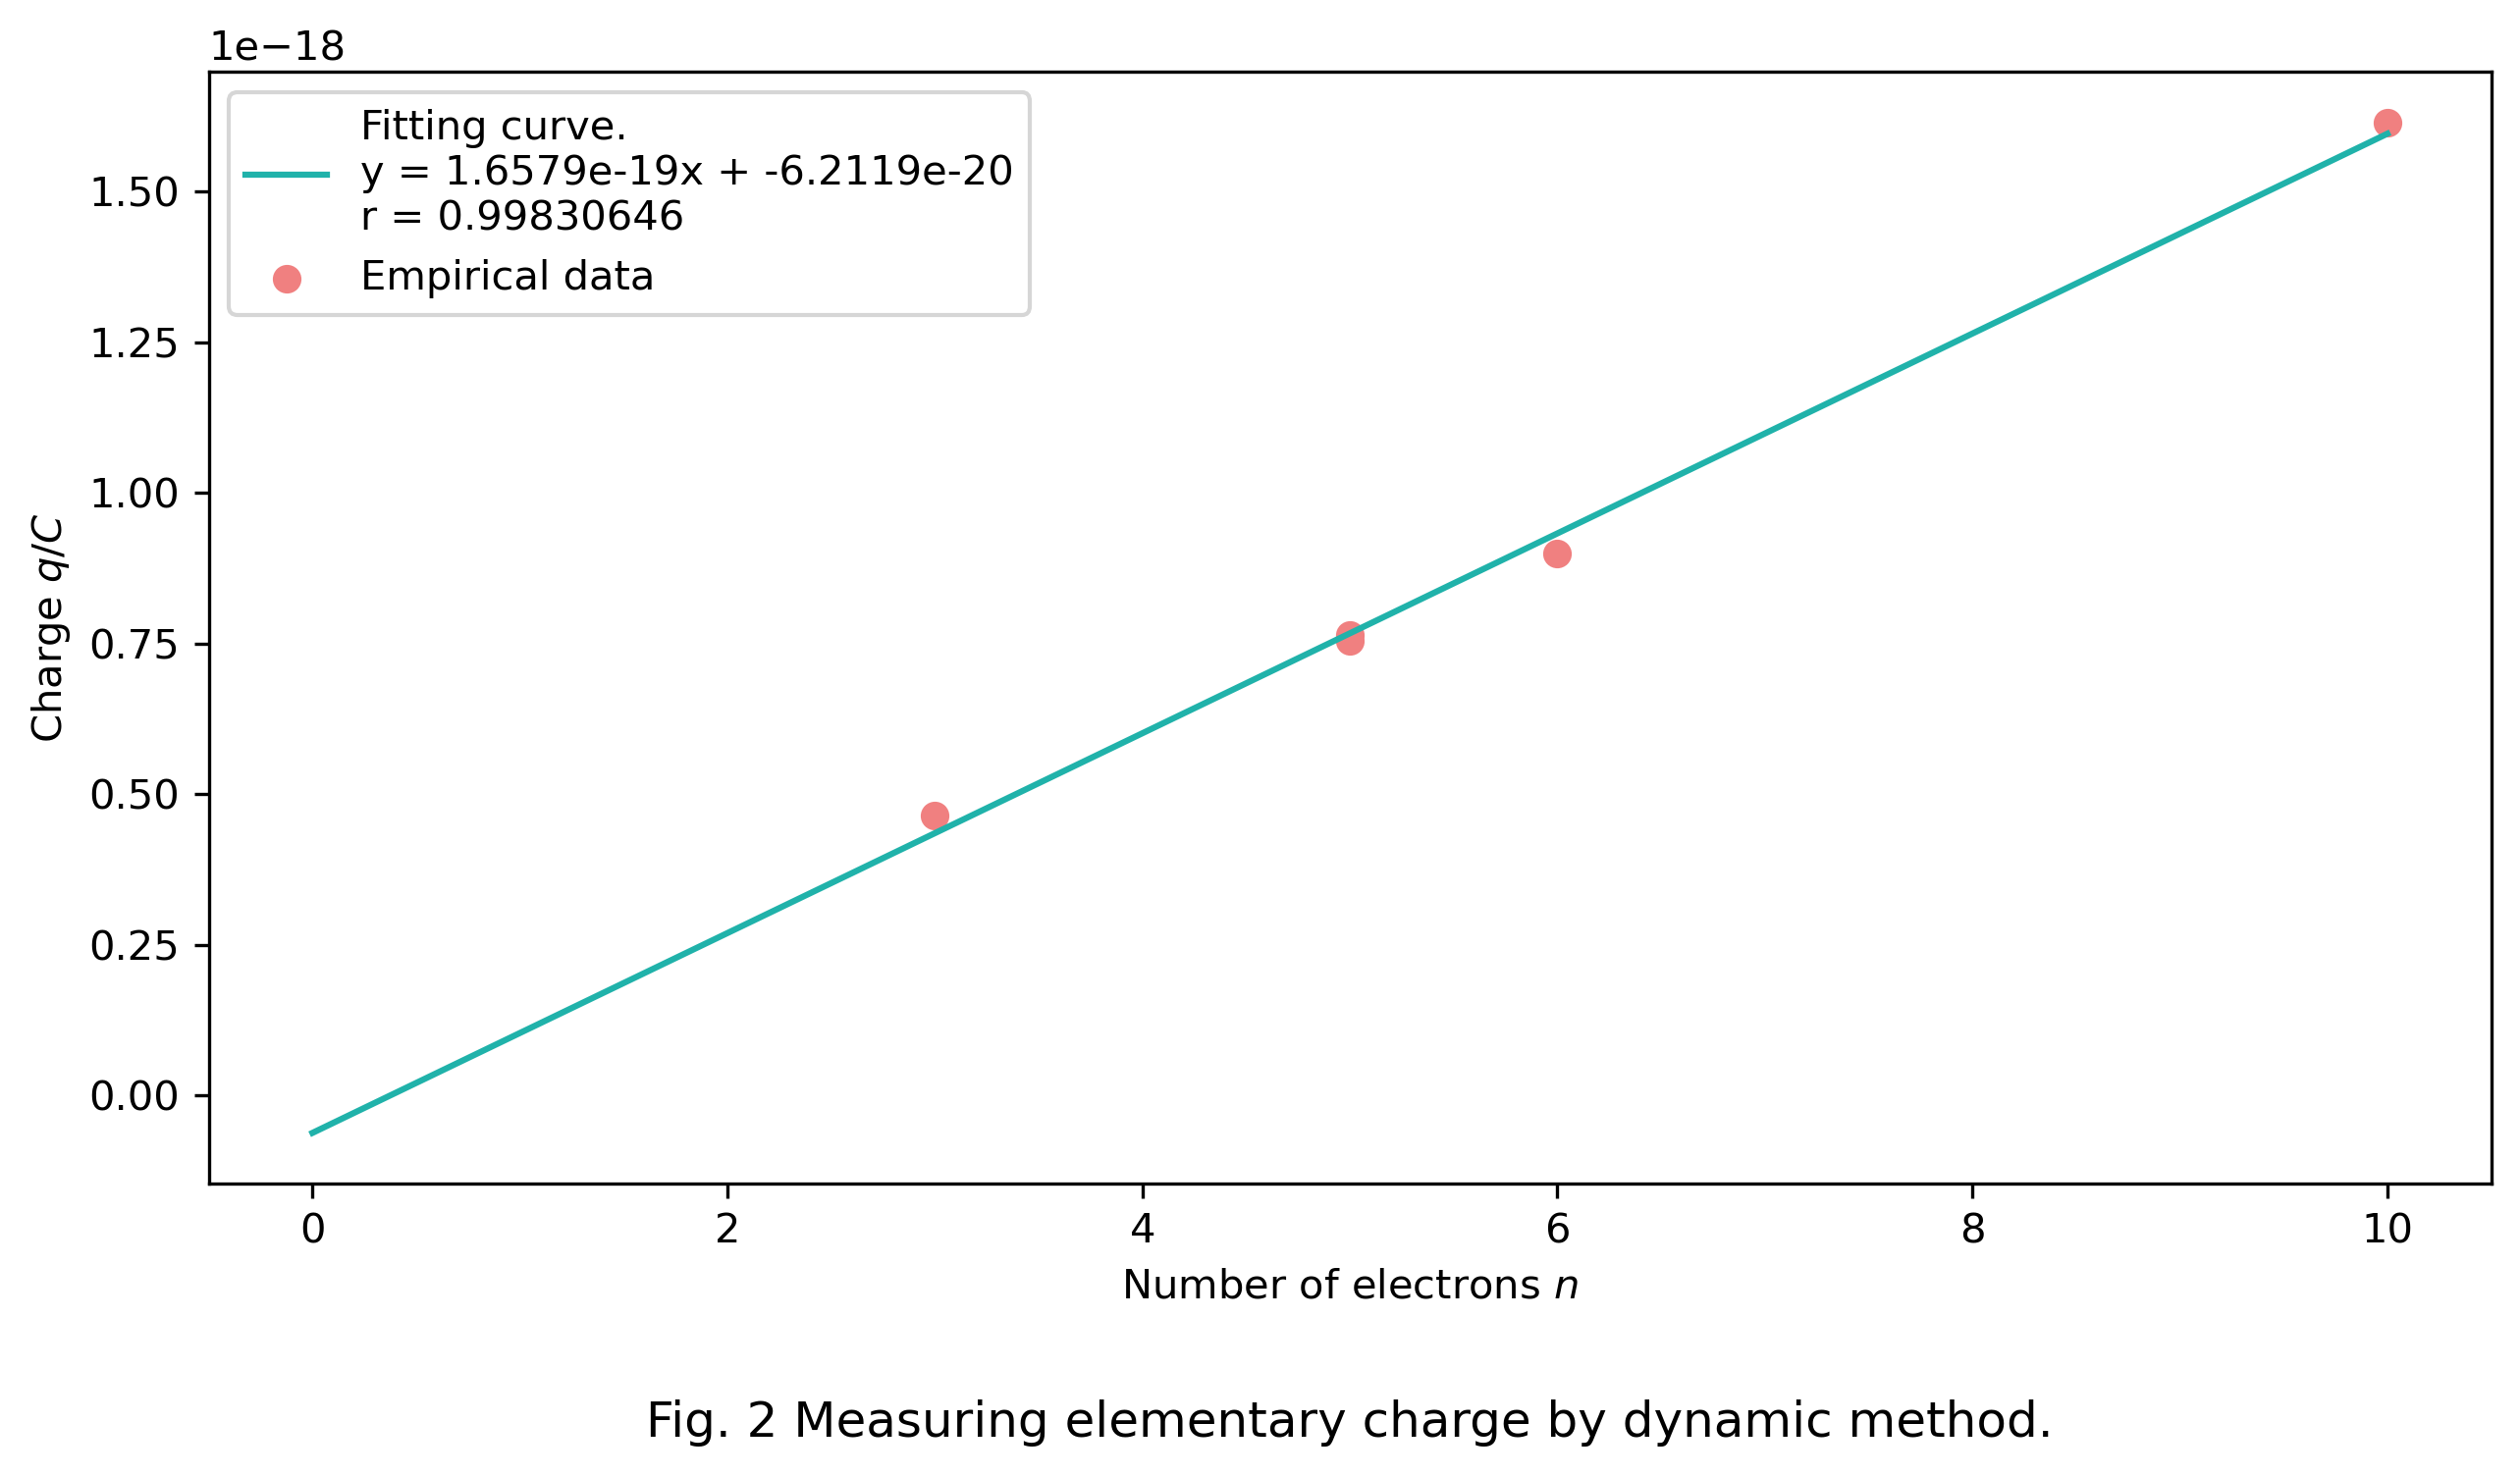
\includegraphics[width=0.7\textwidth]{attachments/fig.2.png}
        \caption{动态法拟合计算元电荷}
        \label{fig:2}
    \end{figure}

    拟合相关系数$r>0.99$,拟合效果好。
    元电荷测量值等于直线斜率$e = 1.66 \times 10^{-19} C$,相对误差为$3.4\%$。
    
    \subsubsection*{3. 实验结果和误差分析}
    实验分别采用动态法和静态法测量油滴带电量,并拟合推算元电荷数值。
    动态法测量元电荷电量数值为$e = 1.61 \times 10^{-19} C$,相对误差为$0.7\%$。
    静态法测量元电荷电量数值为$e = 1.66 \times 10^{-19} C$,相对误差为$3.4\%$。
    
    与动态法相比,静态法测量结果更为精确。分析可能的误差来源有:
    \begin{enumerate}[label=\arabic*.]
        \item 静态法误差主要来源于平衡电压的精确调定。电压调节最小分度只有$1V$,
        由于油滴布朗运动的影响,加上油滴缓慢挥发,事实上很难调整至油滴完全平衡。
        \item 动态法误差主要来源于计时点的精确控制。由于动态法测量要求测量油滴上升和下降时间,
        在切换电压时,由于电路延迟和油滴惯性,油滴很难做完全的匀速运动。
        并且由于需要同时操作电压切换和计时器,依赖于反应时间,会引入较大人为误差。
    \end{enumerate}

\subsection*{【思考题】}
    \subsubsection*{1. 本实验如何通过宏观量测量微观量?}
    本实验通过带电油滴在重力场和电场作用下的平衡运动来建立宏观量和微观量之间的联系。
    可观测的宏观量为油滴的运动状态及工作电压,微观量为油滴尺寸、质量、带电量和电子数等。
    通过观察油滴在其重力和阻力下的平衡运动以及外加电场对电荷运动的影响,依据受力关系可以方便求出油滴的微观量。
    通过大量测量数据统计规律,可以求元电荷数值。

    \subsubsection*{2. 如何保证油滴匀速运动?}
    让油滴在距计时线稍前一段距离开始运动,
    使油滴在到达刻度线时已实现加速,达到最终匀速运动的速度。
    所以实验在视野范围内,应尽可能让油滴开始运动的位置远离计时线。


\subsection*{【项目源码】}
\url{https://github.com/Jeg-Vet/SYSU-PHY-EXP/tree/main/C1-Millikans_oil-drop_experiment}

\end{document}